\documentclass[a4paper,11pt]{article}

\usepackage[english]{babel}
\usepackage[utf8x]{inputenc}
\usepackage{amsmath}
\usepackage{graphicx}
\usepackage{cite}
\usepackage{hyperref}
\usepackage{fullpage}
% \usepackage{apacite}
\setlength{\parskip}{1.2ex}
\begin{document}

\title{Open Information System: Conceptual schema}
\author{Thomas Perale -- 0546990\\Maximilien Romain -- 0543411\\Felipe Rojas -- 0542569\\Lehal Sherik -- 0543118}
\date{27 October 2017}

\maketitle

\section{Project subject}

Our Webowl has eight classes, Category, Ebook, Purchase, Publisher, Author, User, Publisher, Role and Rating.
The User class has eight attributes which are pay information, name, email, password, userID, lastName, two roles "client" and "admin", which are further connected to the Role class.
Purchase class has two attributes ID and Timestamp, and is bounded to User class by "isMaking" relation where the User is the domain and Purchase is the range. The Purchase class is also a master class to the "PaymentMethod" and "DeliveryMethod" classes.


The user class is also bounded to the eBook class, with has four attributes year, version, title and ISBN, by the relation "hasPurchased" and "manage" where the User is the domain and eBook class is the range because of the second rule, that is explained below. The ebook class is also a subclass of "ProductorService" class. The eBook class will related to Purchase class through the relation “isPartOf” where the domain is the ebook class and the range is the purchase class. 
Class named Rating with attributes ID and Number, is connected to eBook with the domain eBook and range Rating and User class with the domain User and range Rating through the relations “hasRating” and “hasRated” respectively.

The eBook class is bounded to Category class, that has two attributes ID and description, by the relation "hasCategory", where domain is ebook and the range is Category. Also the Category class has the relation “subCategoryOf” which infers that an eBook can have two categories, making one of them a subcategory as explained below in the rule one.

The eBook class is also bounded to the Publisher class by the relation "isPublishedby", where Ebook class is the domain and Publisher class is the range. The attributes of the Publisher class are the ID and name and it's also a subclass to "BusinessEntity" class.

The Author class, has three attributes, ID, first name and last name, and is bounded to Ebook class by "hasWritten" where the domain is the Author class and the range is the Ebook class. 

Rules

\section{Rules description}
First rule, If the category of a book is also a subCategory of another category, it implies that the book belongs to both category and subcategory. Example- If a book belongs to "war" category and the "war" category belongs to "action" category, it is implied that the book belongs to both "war" and "action" categories.\\
Ebook(?x), Category(?y), Category(?z), subCategoryOf(?y, ?z), hasCategory(?x, ?y), differentFrom(?y, ?z) $\rightarrow$ hasCategory(?x, ?z)

Second rule, If a user has Purchased an ebook, and the ebook is part of a purchase, then we can imply that the user “HasPurchased” an ebook. \\
User(?x), Purchase(?y), Ebook(?z), isMaking(?x, ?y), isPartOf(?z, ?y) $\rightarrow$ hasPurchased(?x, ?z)

Third rule, If a user has rated an ebook, it implies that the user purchased the ebook as the users can't rate a book without purchasing one. \\

User(?x), Rating(?y), Ebook(?z), hasRating(?x, ?y), hasRating(?z, ?y) $\rightarrow$ hasPurchased(?x, ?z)

The last rule implies that if a user has the role "admin", they can manage the ebooks database on the system. \\
User(?admin), Ebook(?book), AdminRole(?role), hasAdminRole(?admin, ?role) $\rightarrow$ manage(?admin, ?book)

\section{ER Schema}

\begin{center}
  \makebox[\textwidth]{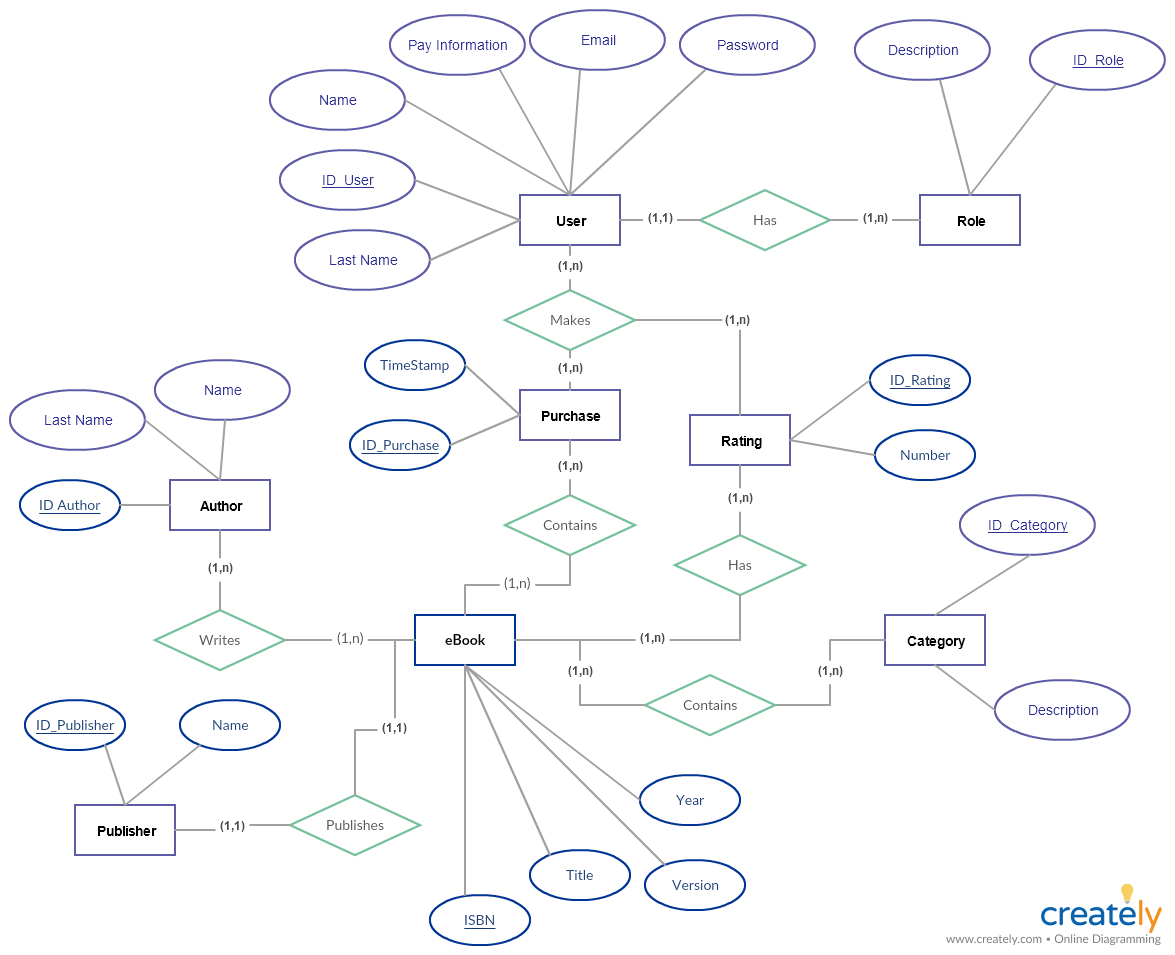
\includegraphics[width=\paperwidth]{ER_graph.png}}
\end{center}

\section{WebOwl visualisation}
\begin{center}
  \makebox[\textwidth]{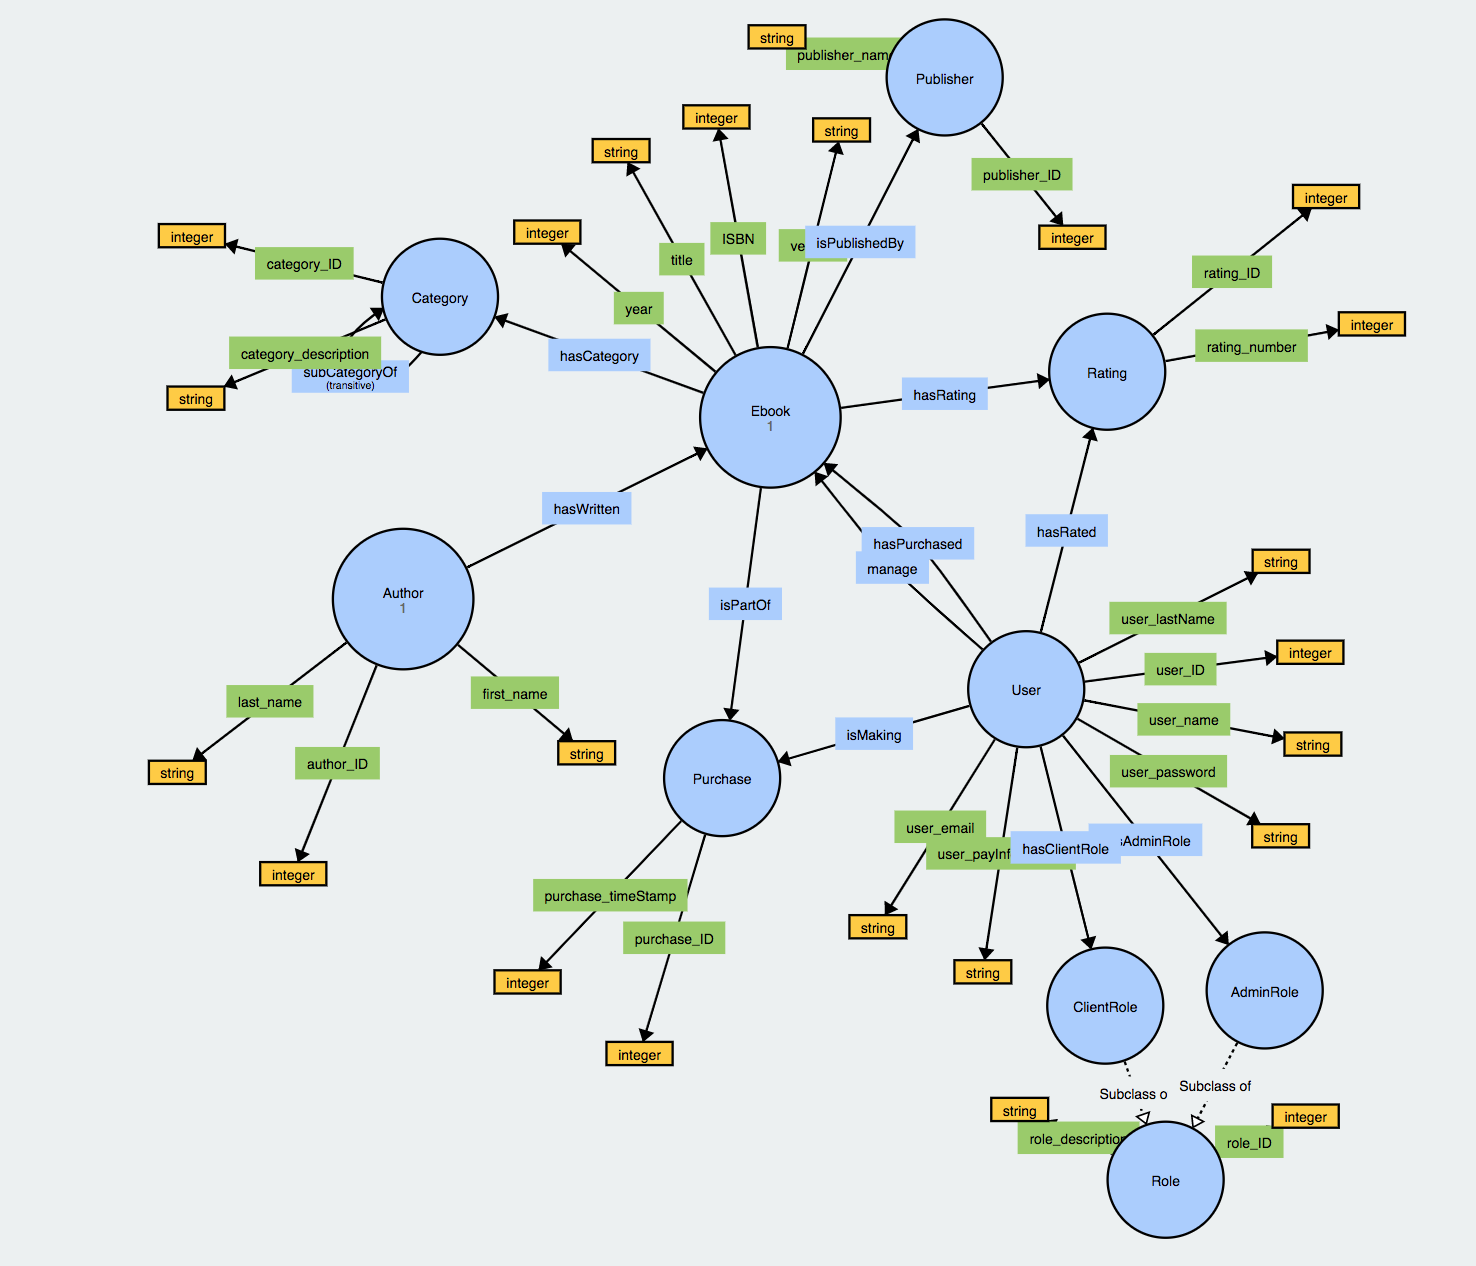
\includegraphics[width=\paperwidth]{webOwl.png}}
\end{center}


\end{document}
